\documentclass[12pt,a4paper]{amsart}
\usepackage[slovene]{babel}
\usepackage[utf8]{inputenc}
\usepackage{amsmath,amssymb,amsfonts}
\usepackage{url}
\usepackage[dvipsnames,usenames]{color}
\usepackage{graphicx}
\usepackage{biblatex}
\usepackage{float}
\usepackage{placeins}

\graphicspath{ {./images/} }
\textwidth 15cm
\textheight 24cm
\oddsidemargin.5cm
\evensidemargin.5cm
\topmargin-5mm
\addtolength{\footskip}{10pt}
\pagestyle{plain}
\overfullrule=15pt 
% ukazi za matematicna okolja
\theoremstyle{definition} % tekst napisan pokoncno
\newtheorem{definicija}{Definicija}[section]
\newtheorem{primer}[definicija]{Primer}
\newtheorem{opomba}[definicija]{Opomba}

\renewcommand\endprimer{\hfill$\diamondsuit$}

\theoremstyle{plain} % tekst napisan posevno
\newtheorem{lema}[definicija]{Lema}
\newtheorem{izrek}[definicija]{Izrek}
\newtheorem{trditev}[definicija]{Trditev}
\newtheorem{posledica}[definicija]{Posledica}

% za stevilske mnozice uporabi naslednje simbole
\newcommand{\R}{\mathbb R}
\newcommand{\N}{\mathbb N}
\newcommand{\Z}{\mathbb Z}
\newcommand{\C}{\mathbb C}
\newcommand{\Q}{\mathbb Q}

% ukaz za slovarsko geslo
\newlength{\odstavek}
\setlength{\odstavek}{\parindent}
\newcommand{\geslo}[2]{\noindent\textbf{#1}\hspace*{3mm}\hangindent=\parindent\hangafter=1 #2}


\newcommand{\imeavtorja}{Ana Marija Kravanja}
\newcommand{\naslovdela}{Min-Graph Equipartition Problem with Simulated Annealing}
\newcommand{\letnica}{2019} 

\begin{document}

% od tod do povzetka ne spreminjaj nicesar
\thispagestyle{empty}
\noindent{\large
UNIVERZA V LJUBLJANI\\[1mm]
FAKULTETA ZA MATEMATIKO IN FIZIKO\\[5mm]}
\vfill

\begin{center}{\large
{\bf \naslovdela}\\[10mm]
{\bf Poročilo}\\[10mm]
Ana Marija Kravanja, Urška Jeranko, Oskar Kregar}\\[1cm]

\end{center}
\vfill

\noindent{\large
Ljubljana, \letnica}
\pagebreak

\tableofcontents

\pagebreak

\section{\textbf{OPIS PROBLEMA}}
V naši projektni nalogi smo reševali problem deljenja grafa z uporabo dveh predpisanih metod. Poljuben graf smo morali razdeliti na dva skoraj enaka dela tako, da je bilo med tema nastalima deloma čim manj povezav. Projekta smo se lotili tako, da smo napisali algoritma požrešne metode (Greedy Method) in metode simuliranega ohlajanja (Simulated Annealing Heuristic), napisali pa smo tudi funkcijo, ki že razdeljen graf nariše in z barvami prikaže optimalno delitev vozlišč. Algoritma smo preizkusili na več različnih grafih in analizirali, kako se metodi obneseta na gostih, redkih ter poljubnih grafih. Pri metodi simuliranega ohlajanja pa smo spreminjali tudi začetno temperaturo in nato primerjali dobljene rešitve med seboj. Da bi bilo naše preizkušanje algoritmov preprostejše smo še napisali funkcijo, ki vrača naključne matrike sosednosti, poljubnih velikosti. \\

Grafe, ki smo jih preučevali, smo v oba algoritma vstavljali v obliki matrike sosednosti, zato smo na začetku definirali: Naj bo $G=(V,E)$ enostaven graf, pri čemer je $V$ množica vozlišč in $E$ množica povezav. Naj bo število vozlišč enako $n$. Definirali smo delitev grafa na dve množici X in Y, pri čemer je $|X| = \lceil \frac{n}{2} \rceil$. Iskali smo minimalno širino bisekcije, to je najmanjše število povezav med $X$ in $Y$ med vsemi možnimi delitvami. \\

\begin{definicija}
Naj bo $G=(V,E)$ enostaven graf in $X,Y \subseteq V$, tako da je $X \cap Y = \emptyset$ in $X \cup Y =V$.
\begin{itemize}
\item Za $x \in X$ označimo z $I(x)$ notranjo vrednost, to je število povezav $(x,z) \in E;z\in X \backslash \{x\}$ . Analogno definiramo $I(y)$ za $y \in Y$.
\item Za $x \in X$ označimo z $O(x)$ zunanjo vrednost, to je število povezav $(x,z) \in E;z\in Y $ . Analogno definiramo $O(y)$ za $y \in Y$.
\item Za $x \in X, y \in Y$ naj bo $\omega(x,y) := \begin{cases} 1,&\text{if} (x,y) \in E\\ 
0, &\text{sicer}\end{cases} $.
\item Za $x \in X, y \in Y$ naj bo $S(x,y):= O(x)-I(x)+O(y)-I(y)-2\omega(x,y)$.
\end{itemize}
\end{definicija}
\bigbreak

\section{\textbf{POŽREŠNA METODA}}
Požrešna metoda je strategija, ki na vsakem posameznem koraku izbere optimalno rešitev s ciljem, da nas to privede do globalno optimalne rešitve. To pomeni, da algoritem izbere rešitev, ki je trenutno najboljša, vendar se pri tem ne ozira na posledice - ne gleda celotne slike. Težava te metode je, da na vsakem koraku izbere le lokalno najboljšo rešitev, samo upamo pa lahko, da je to tudi prava pot do globalnega optimuma. Pogosto torej sploh ne najde najboljše rešitve, povsem mogoče je celo, da nas pripelje do najslabše možne. \\

\subsection{Algoritem požrešne metode}
Začnemo z naključno delitvijo vozlišč grafa na dve skoraj enako veliki množici X in Y. Algoritem zamenja vozlišči na različnih straneh (pri čemer se vse povezave ohranijo), če s tem dobimo boljšo bisekcijo (manjše število povezav med stranema) in se ustavi, ko to ni več možno. Pri menjavi notranje vrednosti postanejo zunanje in obratno, zato dobimo izboljšano bisekcijo le, če je zgoraj definiran $S(x,y)>0$. \\

Vhodni podatki: Graf $G=(V,E), |V|=n$.
\begin{enumerate}
\item Izberemo neključno delitev $(X,Y)$.
\item Izberemo $x\in X, y\in Y$, tako da je $S(x,y)>0$.
\item Zamenjamo vozlišči $x$ in $y$.
\item Ponavljamo 2. in 3. korak, dokler ne obstajata več $x\in X, y\in Y$, da je $S(x,y)>0$.
\end{enumerate}
Izhodni podatki: delitev $(X,Y)$. \\

Algoritma smo se lotili tako, da smo najprej definirali število vozlišč $n$ kot dolžino vhodnega grafa G, ki ga v funkcijo vstavimo kot seznam seznamov, da dobimo matriko sosednosti. Nato smo morebitne enke na diagonali matrike G spremenili v ničle in s tem izbrisali povezave vozlišč s samimi seboj, ki na rezultat tako nimajo vpliva, s tem pa smo preprečili morebitne komplikacije. V naslednjem koraku smo izbrali delitvi X in Y tako, da je v množici X prva polovica vozlišč, v množici Y pa druga polovica, kar je tudi ena od možnih naključnih delitev. Ker to skoraj zagotovo ni optimalna delitev, smo napisali pomožno funkcijo, ki preveri vse možne delitve na način, ki smo ga opisali zgoraj. Uporabili smo for zanki, ki tečeta po vseh elementih množice X in množice Y, da preverimo vse možne delitve. Notranjo in zunanjo vrednost teh dveh množic smo nastavili na 0. Nato smo uporabili še for zanki, ki štejeta povezave znotraj množic X in Y ter med njima in tako računata notranje in zunanje vrednosti. Na ta način dobimo vrednost $S(x,y)$, ki nam pove, ali vozlišči $x\in X$ in $y\in Y$ zamenjamo. Zanka se izvaja, dokler ne obstaja več pozitiven $S(x,y)$, takrat algoritem vrne množici vozlišč X in Y, ki predstavljata optimalno delitev vozlišč.

\newpage

\subsection{Psevdokoda požrešne metode}

Slika prikazuje psevdokodo požrešne metode. Najprej je napisana pomožna funkcija, ki nam šteje povezave znotraj množic X in Y ter med njima, da nam pove, ali je $S(x,y)$ za izbrani vozlišči pozitiven, torej ali se vozlišči splača zamenjati. Druga funkcija pa je dejanska požrešna metoda, ki opravi začetno delitev in skozi while zanko preverja vse možne delitve.

\FloatBarrier
\begin{figure}
  \centering
  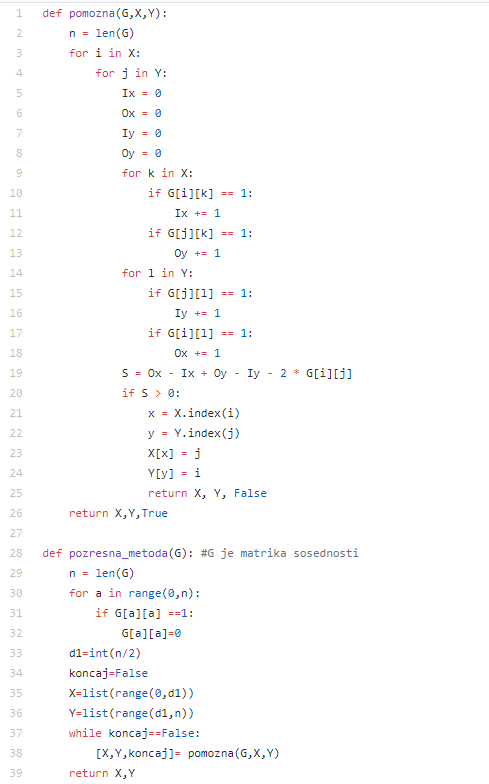
\includegraphics{pozresna}
\end{figure}
\FloatBarrier

\section{\textbf{METODA SIMULIRANEGA OHLAJANJA}}
Algoritem se je v osnovi razvil zaradi procesa toplotne obdelave kovin. Različne materiale segrevamo oz. ohlajamo, da bi spremenili fizikalne lastnosti njihove notranje strukture. Ko se kovina enkrat ohladi, postane njena nova struktura fiksna in kovina tako obdrži pridobljene lastnosti. Pri simuliranem ohlajanju je temperatura naša spremenljivka, ki ponazarja toplotni proces. Na začetku temperaturo nastavimo na visoko vrednost in jo nato sčasoma nižamo, ko se algoritem izvaja. Na začetku, ko je temperatura nastavljena na visoko vrednost, algoritem pogosteje sprejema rešitve, ki so slabše od naše trenutne rešitve zato, da se izogne lokalnim optimumom, ki nas ne bodo pripeljali do globalnega optimuma. Z nižanjem temperature pa se niža tudi verjetnost, da bo algoritem izbiral slabše rešitve; postopoma se torej osredotoči na iskalno območje, na katerem upamo, da je mogoče najti rešitev blizu optimalne. Algoritem je zelo učinkovit pri iskanju rešitev za probleme velikih velikosti, ki vsebujejo številne lokalne optimume.

\subsection{Algoritem metode simuliranega ohlajanja}
Graf definiramo analogno kot pri požrešni metodi. Vozlišči pa zdaj zamenjamo z verjetnostjo $$P(x,y,t) = e^{\frac{Q(R)-Q(S)}{t}}; t\ge 0$$ \\

S $Q(S)$ je označena funkcija, ki množici S priredi neko kvaliteto, torej če je $Q(S) >Q(R)$, pomeni, da je množica S(???) bolj ugodna za nadaljnjo obravnavo.
Za funkcijo $Q$ smo si v našem primeru izbrali število povezav med množicama. Torej če je $Q(R)$ funkcija, kjer smo v množici $R$ zamenjali vozlišča, in $Q(S)$ množica $S$, kjer ju nismo zamenjali, in velja, da je $Q(R)<Q(S)$, potem z določeno verjetnostjo zamenjamo $R$ z $S$. V množici R je v tem primeru med podmnožicama namreč manj povezav kot v S. \\
\begin{enumerate}
\item t = temperatura, ki jo nastavimo na visoko vrednost
\item S = začetna delitev grafa na množici X in Y 
\item N = S  (t.j. trenutna najboljša rešitev)
\item Ponavljaj, dokler je N najboljša rešitev, nam je zmanjkalo časa ali pa je $t \leq 0$:
\item \hspace{1cm} R = delitev, kjer zamenjamo $x\in X$ in $y\in Y$
\item \hspace{1cm} če je $Q(R)<Q(S)$ ali naključno število med 0 in 1, ki je manjše od $P(x,y,t)$, potem je $S=R$
\item \hspace{1cm} zmanjšamo t
\item \hspace{1cm} če je $Q(S)>Q(N)$:
\item \hspace{2cm} $N=S$
\item vrni $N$		\\
\end{enumerate}

Algoritem simuliranega ohlajanja smo napisali kot funkcijo, ki sprejme kot vhodna podatka matriko sosednosti G (seznam seznamov) in temperaturo t, ki jo običajno nastavimo na visoko vrednost (korak 1). Tudi tokrat smo začeli tako, da smo definirali število vozlišč $n$ kot dolžino vhodnega grafa G in morebitne enke na diagonali matrike sosednosti G spremenili v ničle. Ponovno smo definirali začetno delitev tako, da množica X vsebuje prvo polovico vozlišč, množica Y pa drugo polovico (korak 2). Nato smo napisali pomožno funkcijo $seznam\_stevila\_sosedov(G,X,Y)$, ki nam prešteje povezave znotraj množic X in Y ter med njima in poleg števila povezav vrne še začetno število sosedov za vsako vozlišče. Na ta način smo dobili notranje in zunanje vrednosti množic X in Y. V naslednjem koraku smo privzeli, da je trenutna rešitev, to je naša začetna delitev, kar optimalna oz. najboljša rešitev (korak 3). Potem  smo napisali while zanko, ki se izvaja, dokler nismo prekoračili 5000 korakov (časovna omejitev), je temperatura manjša od 0 ali število povezav med množicama vozlišč enako 0, kar se niti ne more zgoditi, če delamo s povezanimi grafi (korak 4). V kolikor pa obravnavamo tudi nepovezane grafe, je to že naša optimalna rešitev. Potem za trenutni seznam števila sosedov in trenutno število povezav (te se bodo spreminjale, ko se zanka izvaja) nastavimo naše najboljše rešitve, ki so zaenkrat kar rešitve začetne delitve. Sledi računanje trenutnega števila povezav za naključno izbrana dva vozlišča iz različnih množic, za kar pa potrebujemo trenutni seznam števila sosedov. Seveda moramo upoštevati tudi, ali sta ta dva vozlišča povezana med seboj. Nato moramo preveriti, ali se vozlišča splača zamenjati. Pri tej metodi to storimo tako, da preverimo, ali je trenutno število povezav manjše od najboljšega števila povezav. Če to ne velja, lahko vozlišči vseeno zamenjamo, če je naključno število med 0 in 1, manjše od $P(x,y,t)$ (korak 6). Če je vsaj eden od zgornjih pogojev izpolnjen, se vozlišči zamenjata, torej se spremenijo tudi sosedi, notranje vrednosti pa postanejo zunanje in obratno. Na koncu še prištejemo korak, da ne prekoračimo časovne omejitve, in znižamo temperaturo, kot narekuje metoda simuliranega ohlajanja. Algoritem vrne optimalni množici vozlišč in število povezav med njima.

\newpage

\subsection{Psevdokoda simuliranega ohlajanja}

Na prvi sliki je prikazana pomožna funkcija, ki vrne seznam seznamov in število povezav med začetnima množicama delitve X in Y. V zunanjem seznamu je toliko elementov, kot je vozlišč v grafu, torej $n$. Prva številka v notranjem seznamu pa za vsako vozlišče pomeni, koliko sosedov ima v svoji množici in koliko jih ima v drugi množici. Ta števila bomo potrebovali pri računanju trenutnega števila povezav pri simuliranem ohlajanju, kar pa je bistvenega pomena. Na naslednji sliki je funkcija simuliranega ohlajanja, ki je odvisna tudi od parametra t, torej temperature. Na enak način kot pri požrešni metodi funkcija opravi začetno delitev na množici X in Y. Računanje števila povezav se izvaja v while zanki, ki teče, dokler je $t>0$ oz. ne presežemo določenega števila korakov. V zanki vozlišča izbiramo naključno in na poseben način preverjamo, ali se ju splača zamenjati. Zadnja funkcija pa je funkcija, ki generira simetrične matrike, katerih elementa sta lahko samo 0 in 1. Te matrike predstavljajo naše naključne matrike sosednosti oz. enostavne grafe.

\FloatBarrier
\begin{figure}
  \centering
  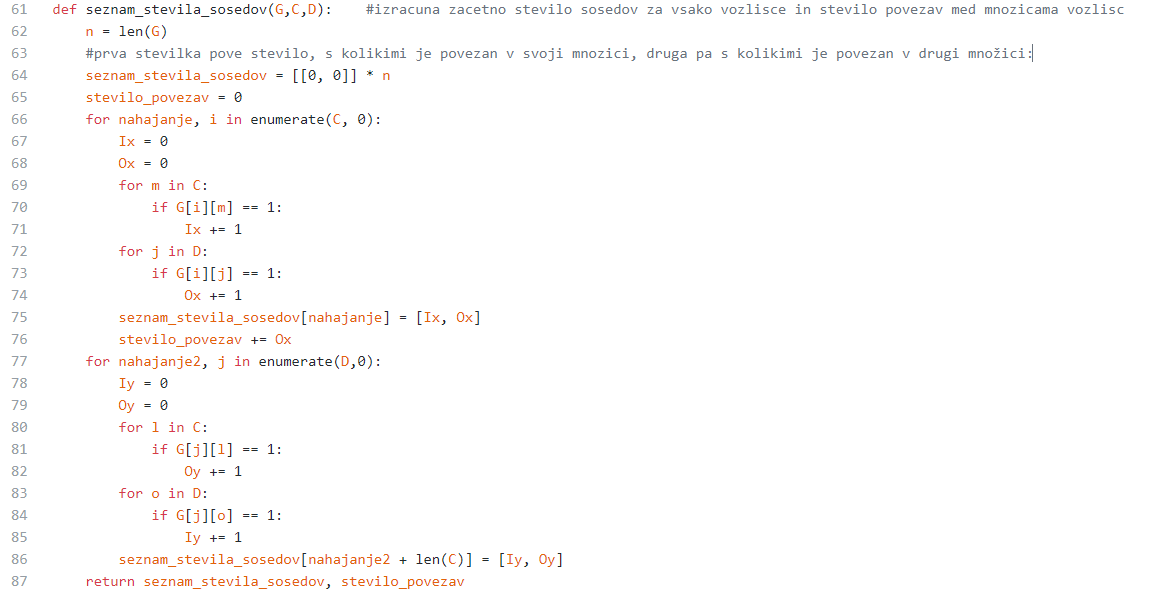
\includegraphics{seznam}
\end{figure}
\FloatBarrier

\FloatBarrier
\begin{figure}
  \centering
  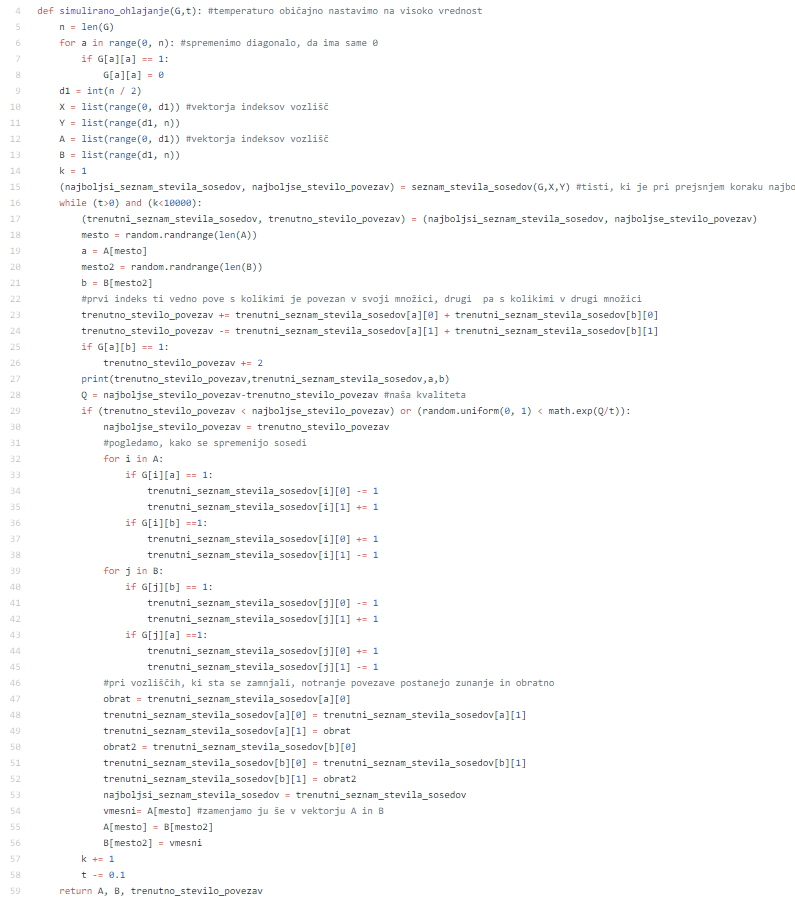
\includegraphics{simulirano}
\end{figure}
\FloatBarrier

\FloatBarrier
\begin{figure}
  \centering
  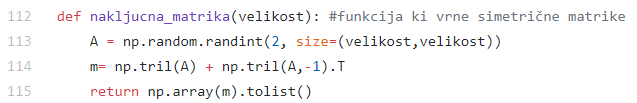
\includegraphics{matrike}
\end{figure}
\FloatBarrier

\newpage

\section{\textbf{SKLEP IN ZAKLJUČEK}}

\newpage

\begin{thebibliography}{9}
\bibitem{integer} 
L. A. Wolsey, Integer Programming, Wiley Interscience,1998. 

 
\bibitem{comparison} 
C. Blum, A. Roli, Metaheuristics in Combinatorial Optimization: Overview and Conceptual Compariosn. [online]
 
\bibitem{metaheuristika} 
S. Luke, Essentials of Metaheuristics: a set of undergraduate lscture notes, online. 

\bibitem{metaheuristika 2}
S. Clinton, Generic algorithms with Python.

\bibitem{metaheuristika2}
K.L. Du, M.N.S. Swamy, Search and optimization by metaheuristics: tehniques and algorithms inspired by nature. 


\bibitem{implementacija}
El. G. Talbi, Metaheuristics: from design to implementation.

\end{thebibliography}




\end{document}
